\subsection{Figures}
\begin{figure}[!htb]
\centering
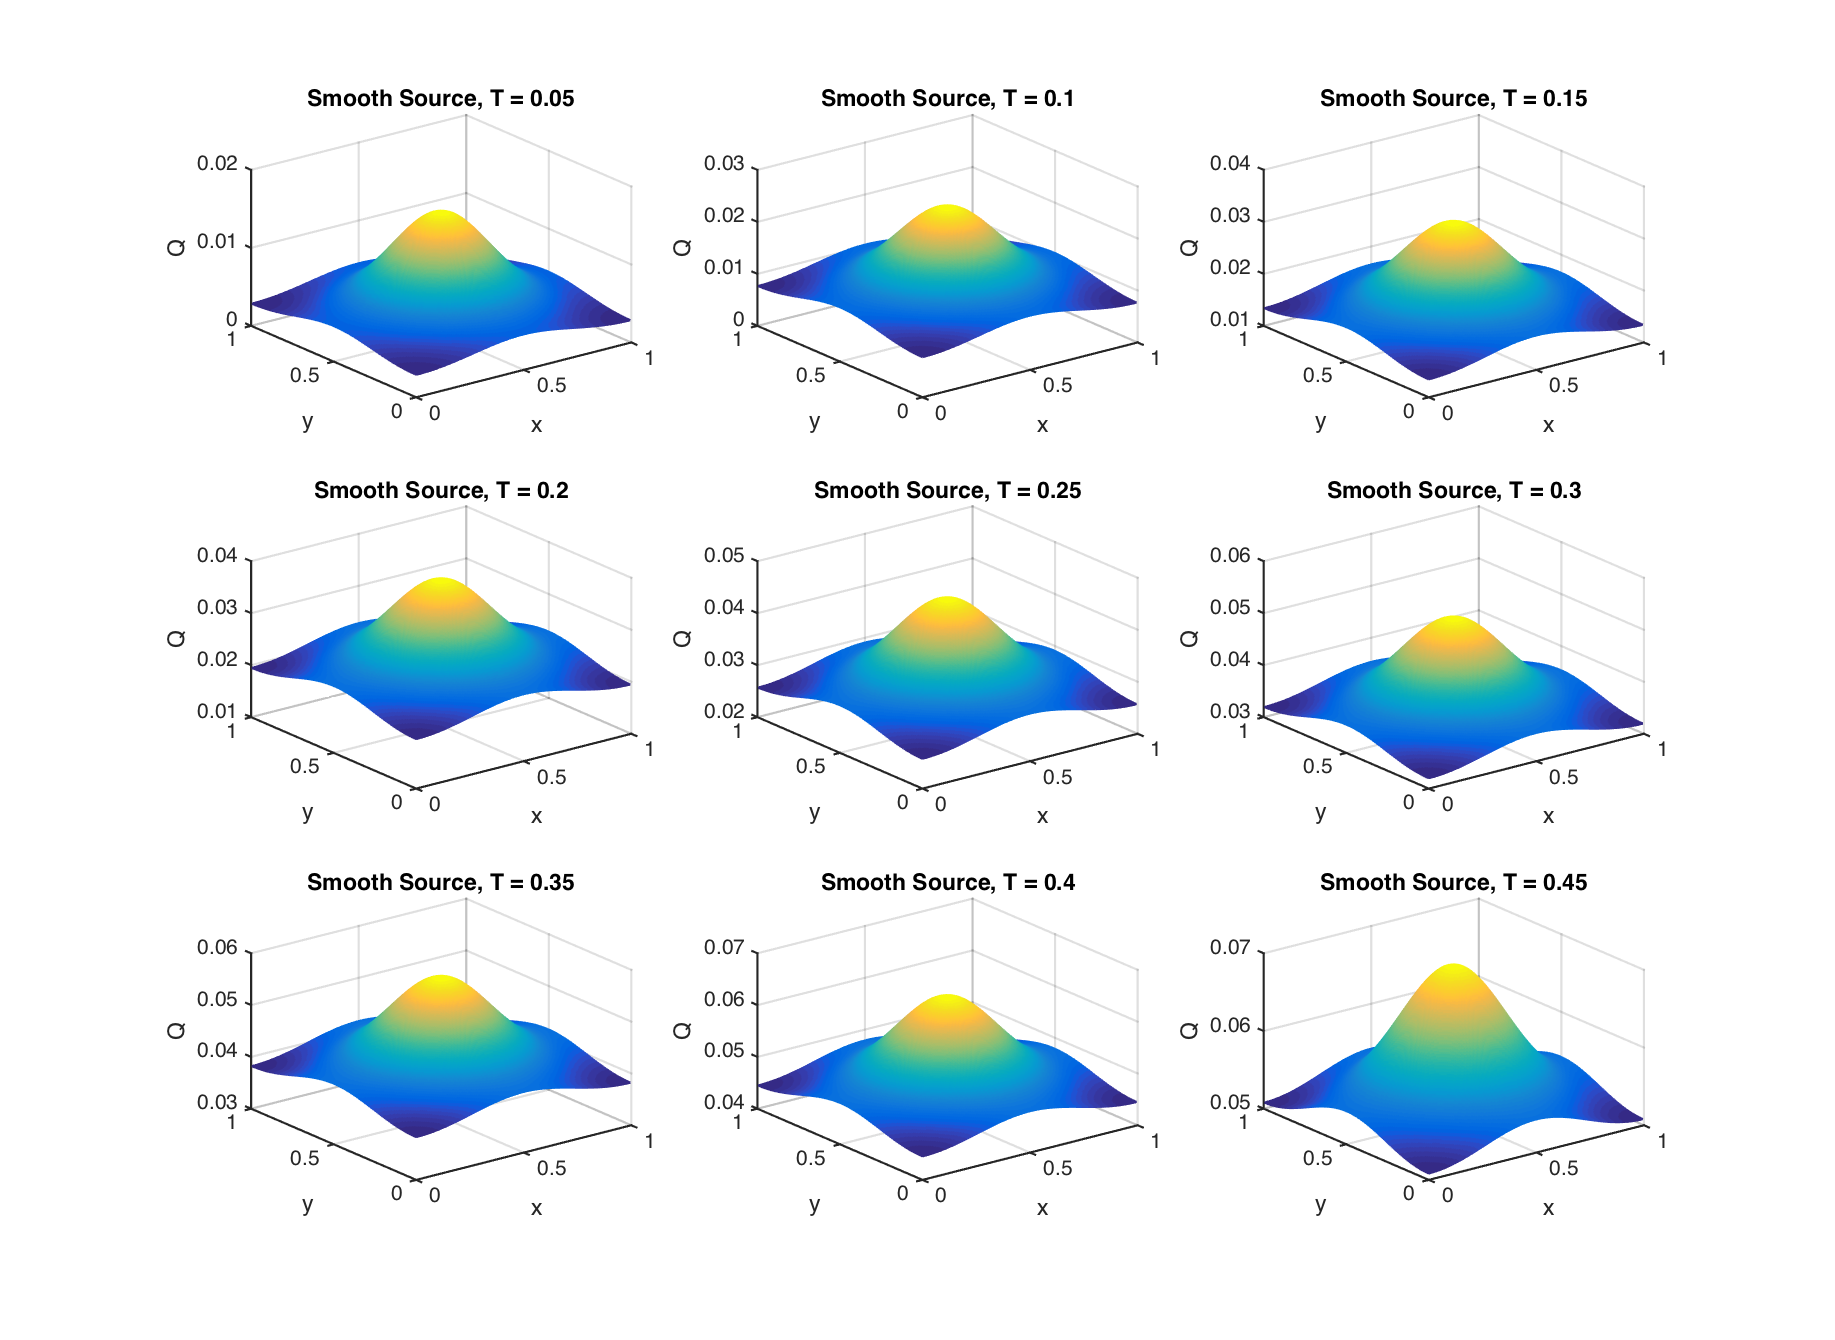
\includegraphics[scale=.5]{smoothSource4_1.eps}
\caption{}
\label{fig:digraph}
\end{figure}

\begin{figure}[!htb]
\centering
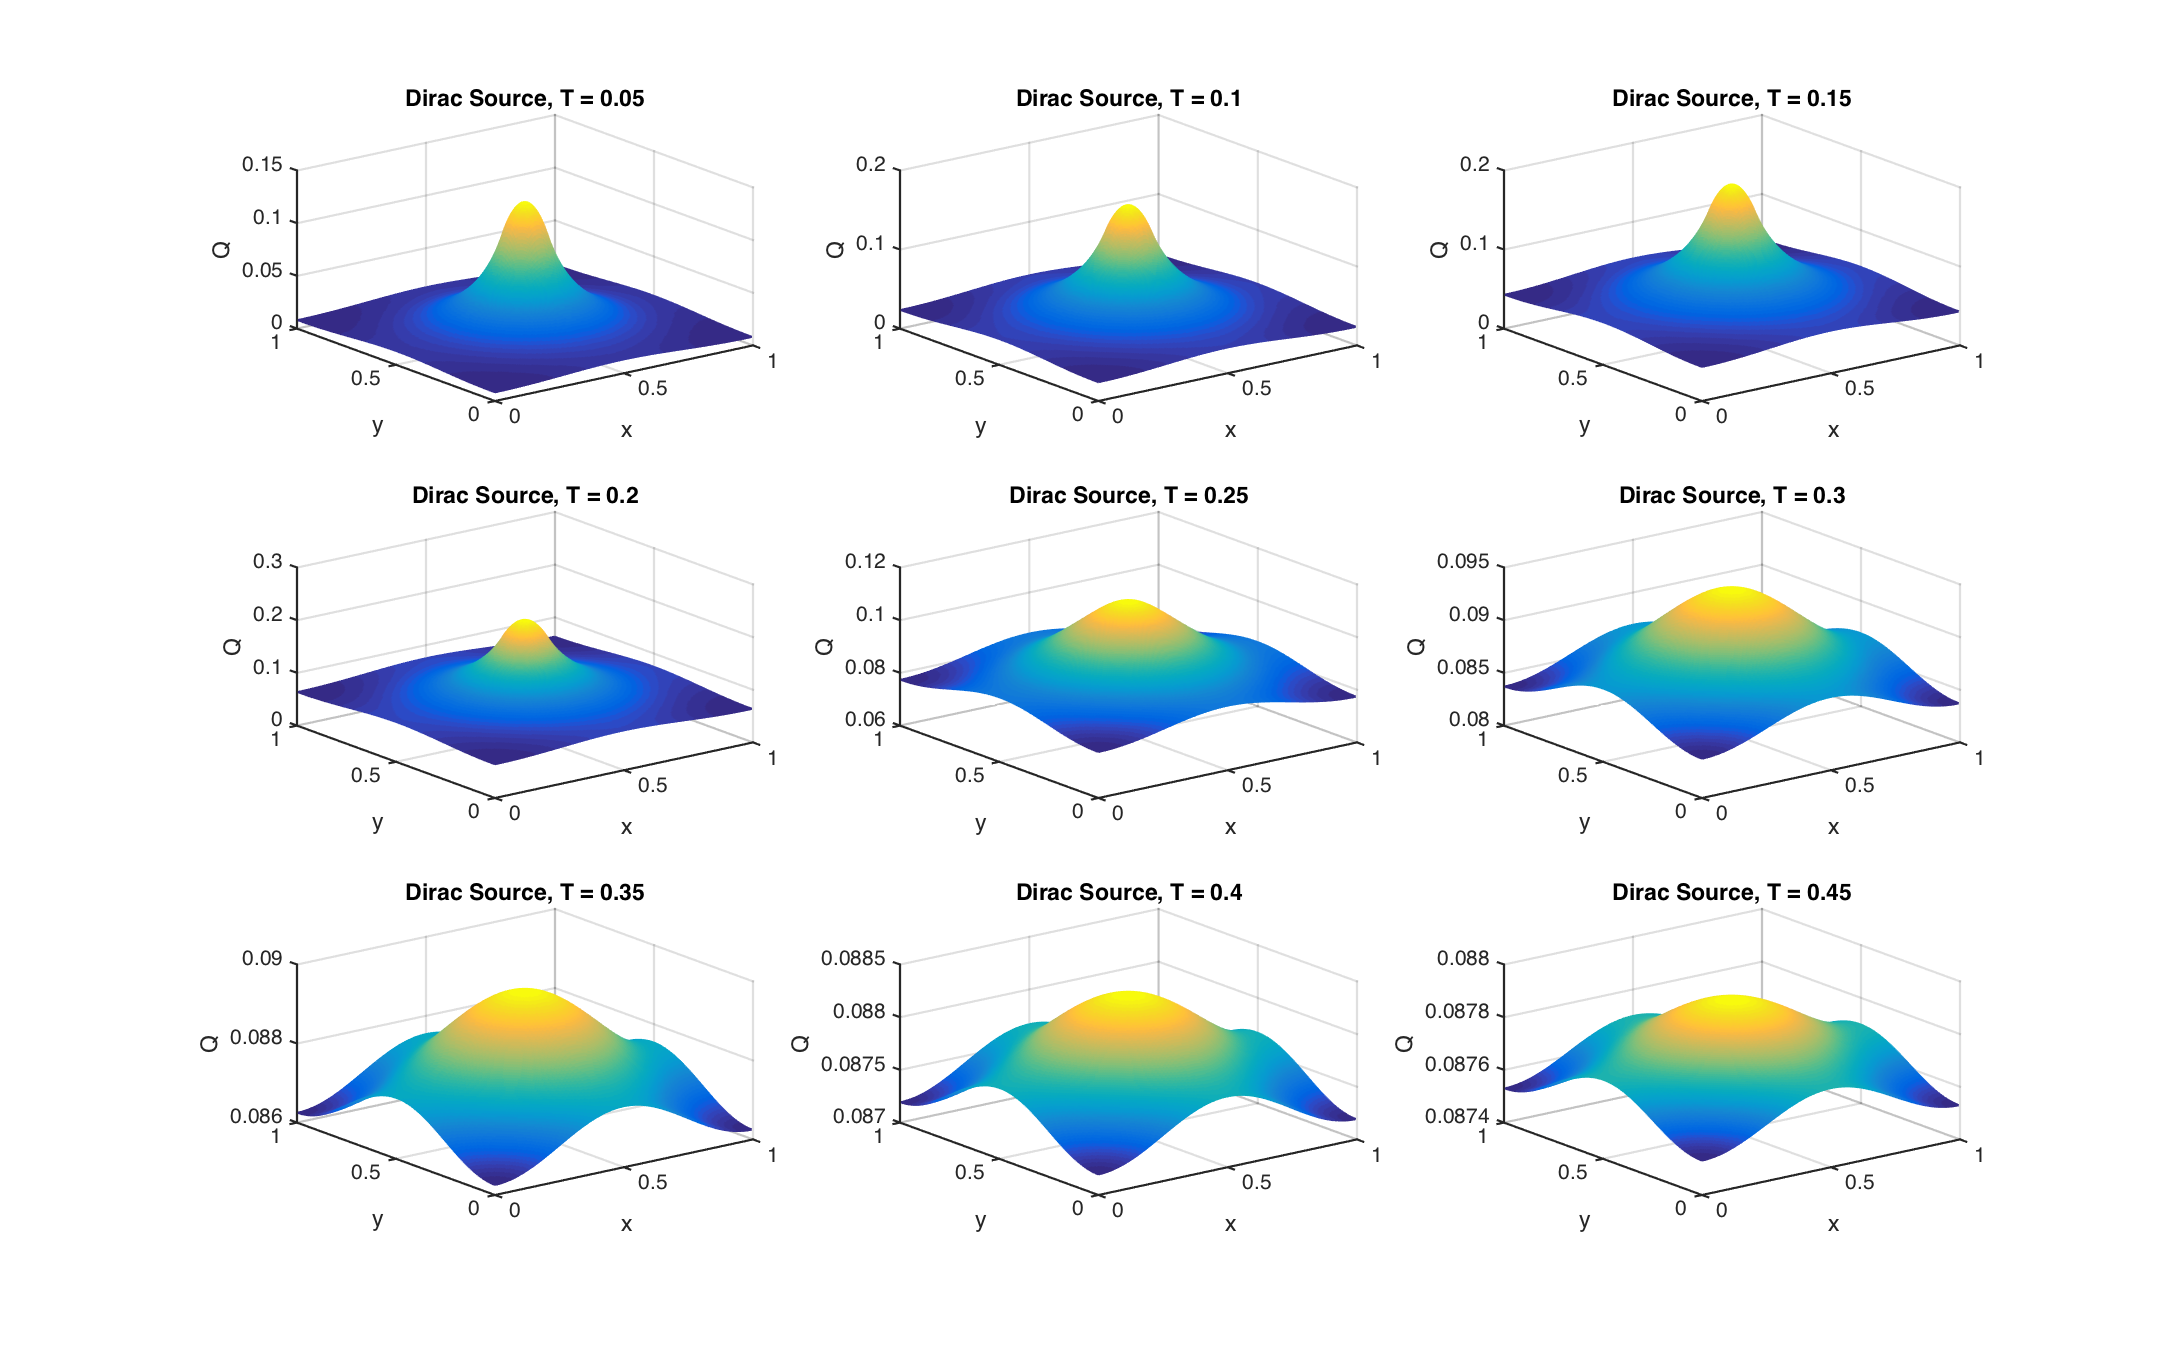
\includegraphics[scale=.5]{diracSource4_1.eps}
\caption{}
\label{fig:digraph}
\end{figure}

\subsection{Convergence}
Because we do not know the true solution to the problem, we study ratios, which we denote by $R$, of the differences of the computed values i.e. 
\begin{align*}
R=\frac{Q'_{h/2,t} - Q'_{h,t}}{Q'_{h/4,t} - Q'_{h/2,t}}
\end{align*}
where, for example, $Q'_{h/2,t}$ is our computed solution using $\Delta x = \Delta y = h/2$ and $\Delta t = t$. We wish to show that the error behaves as $O(\Delta t^p) + O(\Delta h^r)$ and find $p$ and $r$. Letting $Q*$ denote the true solution, we write write our ratio as  
\begin{align*}
R = \frac{Q*+O(\Delta t^p) + O(\Delta (h/2)^r) - (Q* + O(\Delta t^p) + O(\Delta h^r))}{Q*+O(\Delta t^p) + O(\Delta (h/4)^r) - (Q*+O(\Delta t^p) + O(\Delta (h/2)^r))} = \frac{O(\Delta (h/2)^r)-O(\Delta h^r)}{O(\Delta (h/4)^r) - O(\Delta (h/2)^r)}
\end{align*}
We compute several values of R using different h values. We get the following values
\begin{table}[]
\centering
\caption{Order of Convergence in h}
\label{my-label}
\begin{tabular}{|c|c|c|c|}
\hline 
 & h=0.025 & h=0.0125 & 0.00625 \\ 
\hline 
$log_2(R)$ & 1.9962 & 1.9990 & 1.9986 \\ 
\hline 
\end{tabular} 
\\from which we can infer that $r = 2$. We do the same thing in $t$ 
\end{table}